\documentclass[a4paper,11pt]{book}
%\documentclass[a4paper,twoside,11pt,titlepage]{book}
\usepackage{listings}
\usepackage[utf8]{inputenc}
\usepackage[spanish,es-tabla]{babel}

% \usepackage[style=list, number=none]{glossary} %
%\usepackage{titlesec}
%\usepackage{pailatino}

\usepackage{url}
\usepackage{colortbl,longtable}
\usepackage[stable]{footmisc}

\usepackage{minted}

%New colors defined below
\definecolor{codegreen}{rgb}{0,0.6,0}
\definecolor{codegray}{rgb}{0.5,0.5,0.5}
\definecolor{codepurple}{rgb}{0.58,0,0.82}
\definecolor{backcolour}{rgb}{0.95,0.95,0.92}
\definecolor{LightGray}{gray}{0.9}

\definecolor{gray97}{gray}{.97}
\definecolor{gray75}{gray}{.75}
\definecolor{gray45}{gray}{.45}
\definecolor{gray30}{gray}{.94}

\decimalpoint
\usepackage{dcolumn}
\newcolumntype{.}{D{.}{\esperiod}{-1}}
\makeatletter
\addto\shorthandsspanish{\let\esperiod\es@period@code}
\makeatother


%\usepackage[chapter]{algorithm}
\RequirePackage{verbatim}
%\RequirePackage[Glenn]{fncychap}
\usepackage{fancyhdr}
\usepackage{graphicx}
\usepackage{afterpage}

\usepackage{longtable}

\usepackage[pdfborder={000}]{hyperref} %referencia

%Minitoc
\usepackage{minitoc}

% ********************************************************************
% Re-usable information
% ********************************************************************
\newcommand{\myTitle}{Título del proyecto\xspace}
\newcommand{\myDegree}{Master Universitario en Ingeniería de Teñe3comunicación\xspace}
\newcommand{\myName}{Nombre Apllido1 Apellido2 (alumno)\xspace}
\newcommand{\myProf}{Nombre Apllido1 Apellido2 (tutor1)\xspace}
\newcommand{\myOtherProf}{Nombre Apllido1 Apellido2 (tutor2)\xspace}
%\newcommand{\mySupervisor}{Put name here\xspace}
\newcommand{\myFaculty}{Escuela Técnica Superior de Ingenierías Informática y de
Telecomunicación\xspace}
\newcommand{\myFacultyShort}{E.T.S. de Ingenierías Informática y de
Telecomunicación\xspace}
\newcommand{\myDepartment}{Departamento de ...\xspace}
\newcommand{\myUni}{\protect{Universidad de Granada}\xspace}
\newcommand{\myLocation}{Granada\xspace}
\newcommand{\myTime}{\today\xspace}
\newcommand{\myVersion}{Version 0.1\xspace}


\hypersetup{
pdfauthor = {\myName (email (en) ugr (punto) es)},
pdftitle = {\myTitle},
pdfsubject = {},
pdfkeywords = {palabra_clave1, palabra_clave2, palabra_clave3, ...},
pdfcreator = {LaTeX con el paquete ....},
pdfproducer = {pdflatex}
}

%\hyphenation{}


%\usepackage{doxygen/doxygen}
%\usepackage{pdfpages}
\usepackage{url}
\usepackage{colortbl,longtable}
\usepackage[stable]{footmisc}
%\usepackage{index}

%\makeindex
%\usepackage[style=long, cols=2,border=plain,toc=true,number=none]{glossary}
% \makeglossary

% Definición de comandos que me son tiles:
%\renewcommand{\indexname}{Índice alfabético}
%\renewcommand{\glossaryname}{Glosario}

\pagestyle{fancy}
\fancyhf{}
\fancyhead[LO]{\leftmark}
\fancyhead[RE]{\rightmark}
\fancyhead[RO,LE]{\textbf{\thepage}}
\renewcommand{\chaptermark}[1]{\markboth{\textbf{#1}}{}}
\renewcommand{\sectionmark}[1]{\markright{\textbf{\thesection. #1}}}

\setlength{\headheight}{1.5\headheight}

\newcommand{\HRule}{\rule{\linewidth}{0.5mm}}
%Definimos los tipos teorema, ejemplo y definición podremos usar estos tipos
%simplemente poniendo \begin{teorema} \end{teorema} ...
\newtheorem{teorema}{Teorema}[chapter]
\newtheorem{ejemplo}{Ejemplo}[chapter]
\newtheorem{definicion}{Definición}[chapter]

\definecolor{gray97}{gray}{.97}
\definecolor{gray75}{gray}{.75}
\definecolor{gray45}{gray}{.45}
\definecolor{gray30}{gray}{.94}

\lstset{ frame=Ltb,
     framerule=0.5pt,
     aboveskip=0.5cm,
     framextopmargin=3pt,
     framexbottommargin=3pt,
     framexleftmargin=0.1cm,
     framesep=0pt,
     rulesep=.4pt,
     backgroundcolor=\color{gray97},
     rulesepcolor=\color{black},
     %
     stringstyle=\ttfamily,
     showstringspaces = false,
     basicstyle=\scriptsize\ttfamily,
     commentstyle=\color{gray45},
     keywordstyle=\bfseries,
     %
     numbers=left,
     numbersep=6pt,
     numberstyle=\tiny,
     numberfirstline = false,
     breaklines=true,
   }

% minimizar fragmentado de listados
%\lstnewenvironment{listing}[1][]
%   {\lstset{#1}\pagebreak[0]}{\pagebreak[0]}

\lstdefinestyle{CodigoC}
   {
	basicstyle=\scriptsize,
	frame=single,
	language=C,
	numbers=left
   }
\lstdefinestyle{CodigoC++}
   {
	basicstyle=\small,
	frame=single,
	backgroundcolor=\color{gray30},
	language=C++,
	numbers=left
   }


\lstdefinestyle{Consola}
   {basicstyle=\scriptsize\bf\ttfamily,
    backgroundcolor=\color{gray30},
    frame=single,
    numbers=none
   }


\newcommand{\bigrule}{\titlerule[0.5mm]}


%Para conseguir que en las páginas en blanco no ponga cabecerass
\makeatletter
\def\clearpage{%
  \ifvmode
    \ifnum \@dbltopnum =\m@ne
      \ifdim \pagetotal <\topskip
        \hbox{}
      \fi
    \fi
  \fi
  \newpage
  \thispagestyle{empty}
  \write\m@ne{}
  \vbox{}
  \penalty -\@Mi
}
\makeatother

\usepackage{pdfpages}

% acronyms
\usepackage{acronym} 
% minitoc para cada capítulo
%\usepackage{minitoc}

\begin{document}
\dominitoc
\begin{titlepage}


\newlength{\centeroffset}
\setlength{\centeroffset}{-0.5\oddsidemargin}
\addtolength{\centeroffset}{0.5\evensidemargin}
\thispagestyle{empty}

\noindent\hspace*{\centeroffset}\begin{minipage}{\textwidth}

\centering

\includegraphics[width=0.9\textwidth]{imagenes/logo_ugr.jpg}\\[1.2cm]

%\textsc{ \Large TRABAJO FIN DE MÁSTER\\[0.2cm]}
\textsc{ \Large TRABAJO FIN DE GRADO\\[0.2cm]}
%\textsc{INGENIERÍA INFORMÁTICA}\\[1cm]
\textsc{INGENIERÍA DE TECNOLOGÍAS DE TELECOMUNICACIÓN}\\[1cm]
% Upper part of the page
%
% Title
{\Huge\bfseries Titulo del Proyecto\\
}
\noindent\rule[-1ex]{\textwidth}{3pt}\\[3.5ex]
{\large\bfseries Subtitulo del Proyecto}
\end{minipage}

\vspace{2.5cm}
\noindent\hspace*{\centeroffset}\begin{minipage}{\textwidth}
\centering

\textbf{Autor}\\ {Nombre Apellido1 Apellido2}\\[2.5ex]
\textbf{Directores}\\
{Nombre Apellido1 Apellido2\\
Nombre Apellido1 Apellido2}\\[2cm]

\includegraphics[width=0.3\textwidth]{imagenes/etsiit_logo.png}\\[0.1cm]
\textsc{Escuela Técnica Superior de Ingenierías Informática y de Telecomunicación}\\
\textsc{---}\\
Granada, mes de 202
\end{minipage}
%\addtolength{\textwidth}{\centeroffset}
%\vspace{\stretch{2}}
\end{titlepage}



\chapter*{}
%\thispagestyle{empty}
%\cleardoublepage

%\thispagestyle{empty}

\begin{titlepage}
 
 
\setlength{\centeroffset}{-0.5\oddsidemargin}
\addtolength{\centeroffset}{0.5\evensidemargin}
\thispagestyle{empty}

\noindent\hspace*{\centeroffset}\begin{minipage}{\textwidth}

\centering
%
\includegraphics[width=0.9\textwidth]{imagenes/logo_ugr.jpg}\\[1.4cm]

%\textsc{ \Large PROYECTO FIN DE CARRERA\\[0.2cm]}
%\textsc{ INGENIERÍA EN INFORMÁTICA}\\[1cm]
% Upper part of the page
% 

 \vspace{3.3cm}

%si el proyecto tiene logo poner aquí

\includegraphics[width=0.9\textwidth]{imagenes/logo_ugr.jpg} 
 \vspace{0.5cm}

% Title

{\Huge\bfseries Título del proyecto\\
}
\noindent\rule[-1ex]{\textwidth}{3pt}\\[3.5ex]
{\large\bfseries Subtítulo del proyecto.\\[4cm]}
\end{minipage}

\vspace{2.5cm}
\noindent\hspace*{\centeroffset}\begin{minipage}{\textwidth}
\centering

\textbf{Autor}\\ {Nombre Apellido1 Apellido2}\\[2.5ex]
\textbf{Directores}\\
{Nombre Apellido1 Apellido2\\
Nombre Apellido1 Apellido2}\\[2cm]
%\includegraphics[width=0.15\textwidth]{imagenes/tstc.png}\\[0.1cm]
%\textsc{Departamento de Teoría de la Señal, Telemática y Comunicaciones}\\
%\textsc{---}\\
%Granada, mes de 201
\end{minipage}
%\addtolength{\textwidth}{\centeroffset}
\vspace{\stretch{2}}

 
\end{titlepage}






\cleardoublepage
\thispagestyle{empty}

\begin{center}
{\large\bfseries Título del Proyecto: Subtítulo del proyecto}\\
\end{center}
\begin{center}
Nombre Apellido1 Apellido2 del alumno\\
\end{center}

%\vspace{0.7cm}
\noindent{\textbf{Palabras clave}: palabra\_clave1, palabra\_clave2, palabra\_clave3, ......}\\

\vspace{0.7cm}
\noindent{\textbf{Resumen}}\\

Poner aquí el resumen.
\cleardoublepage


\thispagestyle{empty}


\begin{center}
{\large\bfseries Project Title: Project Subtitle}\\
\end{center}
\begin{center}
Student's first name and Family name\\
\end{center}

%\vspace{0.7cm}
\noindent{\textbf{Keywords}: Keyword1, Keyword2, Keyword3, ....}\\

\vspace{0.7cm}
\noindent{\textbf{Abstract}}\\

Write here the abstract in English.

\chapter*{}
\thispagestyle{empty}

\noindent\rule[-1ex]{\textwidth}{2pt}\\[4.5ex]

Yo, \textbf{Nombre Apellido1 Apellido2}, alumno de la titulación TITULACIÓN de la \textbf{Escuela Técnica Superior
de Ingenierías Informática y de Telecomunicación de la Universidad de Granada}, con DNI XXXXXXXXX, autorizo la
ubicación de la siguiente copia de mi Trabajo Fin de Master en la biblioteca del centro para que pueda ser
consultada por las personas que lo deseen.

\vspace{6cm}

\noindent Fdo: Nombre Apellido1 Apellido2

\vspace{2cm}

\begin{flushright}
Granada a X de mes de 202 .
\end{flushright}


\chapter*{}
\thispagestyle{empty}

\noindent\rule[-1ex]{\textwidth}{2pt}\\[4.5ex]

D. \textbf{Nombre Apellido1 Apellido2 (tutor1)}, Profesor del Área de XXXX del Departamento YYYY de la Universidad de Granada.

\vspace{0.5cm}

D. \textbf{Nombre Apellido1 Apellido2 (tutor2)}, Profesor del Área de XXXX del Departamento YYYY de la Universidad de Granada.


\vspace{0.5cm}

\textbf{Informan:}

\vspace{0.5cm}

Que el presente trabajo, titulado \textit{\textbf{Título del proyecto, Subtítulo del proyecto}},
ha sido realizado bajo su supervisión por \textbf{Nombre Apellido1 Apellido2 (alumno)}, y autorizamos la defensa de dicho trabajo ante el tribunal
que corresponda.

\vspace{0.5cm}

Y para que conste, expiden y firman el presente informe en Granada a X de mes de 202 .

\vspace{1cm}

\textbf{Los directores:}

\vspace{5cm}

\noindent \textbf{Nombre Apellido1 Apellido2 (tutor1) \ \ \ \ \ Nombre Apellido1 Apellido2 (tutor2)}

\chapter*{Agradecimientos}
\thispagestyle{empty}

       \vspace{1cm}


Poner aquí agradecimientos...


% Con este comando hacemos que los números de las páginas aparezcan en romano y que los capítulos no se enumeren, pese a esto, el título de cada capítulo aparecerá en el índice
\frontmatter

% Con esto creamos el índice
\tableofcontents

% Con esto creamos de forma automática una lista de las figuras y de las tablas
\listoffigures 
\listoftables

% Con mainmatter reseteamos los cambios de frontmatter y se resetea la cuenta de los números de página
\mainmatter

% Con esto hacemos que los párrafos aparezcan separados
\setlength{\parskip}{5pt}

\chapter*{Acrónimos}\addcontentsline{toc}{chapter}{Acrónimos}
\begin{acronym}[MPC] % Give the longest label here so that the list is nicely aligned
\acro{PLC}{Programmable Logic Controller}
\end{acronym}

\input{capitulos/01_Introducción}
%
\chapter{Planificación}\label{cap:planif}

\section{Requisitos}
[Sobre todo en proyectos de diseño software/hardware]

\section{Tareas}
[A partir de los objetivos planteados del proyecto se definirán tareas así como su duración. Un objetivo, puede dar lugar a más de una tarea para su consecución. Es importante relacionar cada tarea con sus objetivos asociados.]

\begin{itemize}
    \item \textbf{Estudio del estado del arte.} ...
    \item \textbf{Evaluación de la propuesta} 
\end{itemize}

\section{Recursos humanos y técnicos}

Los recursos necesitamos para llevar a cabo el proyecto son:

\begin{itemize}
    \item \textbf{Hardware}:
    
    \begin{itemize}
        \item Ordenador de sobremesa HP Z2 SFF G4 Workstation del Laboratorio de Ciberseguridad de la UGR.
        
        \item 2 Raspberries Pi, modelos 4 y 5.
        
        \item Ordenador portátil HP Laptop 15s-eq1xxx.
    \end{itemize}
        
    \item \textbf{Software}:
        
    \begin{itemize}
        \item Sistema operativo Ubuntu 18.04 LTS. Será la distribución Linux principal con la que vamos a trabajar, tanto en forma nativa como en máquinas virtuales.
        
        \item Sistema operativo Raspberry Pi OS Raspbian. Será la distribución Linux con la que vamos a trabajar en las Raspberries Pi.
        
        \item VirtualBox. Con él crearemos máquinas virtuales.
        
        \item \ac{OvS}. Permitirá implementar un switch OpenFlow utilizado en nuestra arquitectura de red.
        
        \item RYU Controller. Es el software elegido para el controlador SDN. Aporta aplicaciones SDN de ejemplo con las que vamos a trabajar.
        
        \item MySQL. Permite usar bases de datos SQL.
        
        \item Grafana. Permite crear representaciones gráficas de datos almacenados en bases de datos de cualquier tipo. Lo utilizaremos junto a MySQL.
        
        \item Mosquitto y Mosquitto-clients. Con mosquitto podremos implementar un \textit{broker} MQTT, y con mosquitto-clients podemos publicar y suscribirnos a diferentes tópicos usando MQTT.
        
    \end{itemize}
    
    \item \textbf{Recursos humanos}. En la Tabla~\ref{table:recursos-humanos} se muestra una aproximación de las horas de trabajo empleadas en las diferentes tareas realizadas, tanto por el desarrollador como por el supervisor, incluyendo las reuniones asociadas a cada tarea.
\end{itemize}

\section{Temporización}

Para alcanzar los objetivos de cualquier proyecto, es necesario llevar a cabo una planificación temporal de las diferentes tareas a realizar.\\

En nuestro caso, no hemos dispuesto de todos los recursos desde el primer momento, por lo que hemos ido adaptando las tareas conforme a lo que podíamos llevar a cabo. La duración de cada tarea depende de varias aspectos como su complejidad y disposición de recursos.\\

Las diferentes tareas que hemos llevado a cabo las mostramos en el diagrama de Gantt donde hemos realizado una planificación por semanas (ver Figura~\ref{fig:gantt}).\\

Para controlar que estas tareas se cumplen en los plazos establecidos, se han llevado a cabo diferentes reuniones con el tutor en las cuales se exponía el trabajo realizado y se determinaban las siguientes tareas a llevar a cabo.\\

\begin{table}[t!]
\begin{tabular}{|c|c|c|}
\hline
\textbf{Tarea} & \textbf{\begin{tabular}[c]{@{}c@{}}Tiempo empleado \\ por el \\ desarrollador (horas)\end{tabular}} & \textbf{\begin{tabular}[c]{@{}c@{}}Tiempo empleado \\ por el \\ tutor (horas)\end{tabular}} \\ \hline
Estado del arte & 25 & 5 \\ \hline
Análisis de las soluciones & 30 & 7 \\ \hline
Diseño e implementación & 60 & 6 \\ \hline
Evaluación de seguridad & 20 & 5 \\ \hline
Securización del sistema & 15 & 2 \\ \hline
\textbf{Total} & \textbf{150} & \textbf{25} \\ \hline
\end{tabular}
\caption{Resumen recursos humanos.}
\label{table:recursos-humanos}
\end{table}

\begin{figure}[t!]
    \centering
    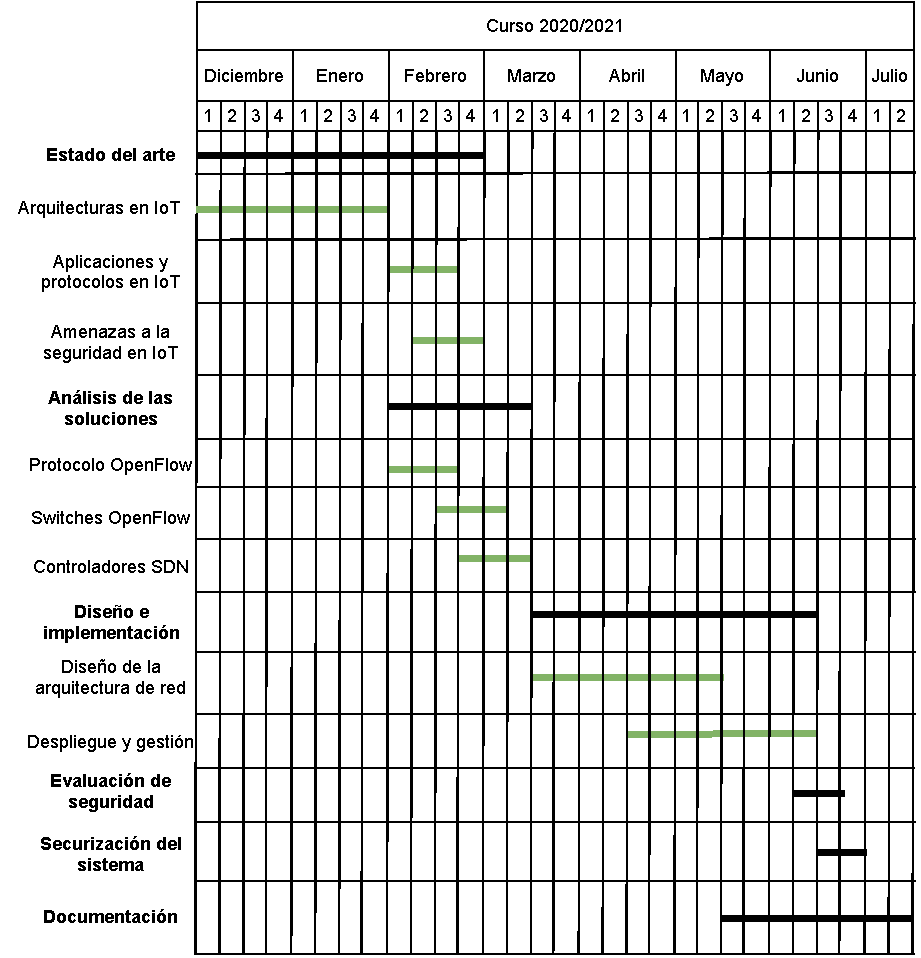
\includegraphics[width=1\textwidth]{imagenes/cap2/gannt.pdf}
    \caption{Diagrama de Gantt del proyecto.}
    \label{fig:gantt}
\end{figure}

\section{Presupuesto}

Para dar un valor económico a este proyecto, tendremos en cuenta los recursos necesarios y el tiempo empleado en el desarrollo de las tareas. Para hacer una aproximación del tiempo empleado, podemos basarnos en el diagrama de Gantt de la Figura~\ref{fig:gantt}.\\

En cuanto a los recursos humanos, el coste del desarrollador será de 25 euros por hora. El proyecto ha estado supervisado por un tutor. Con el tutor se han concertado reuniones cada dos semanas durante los primeros 2 meses y cada semana durante el resto, de una duración media de 30 minutos. El coste de la supervisión es de 70 euros por hora. En la Tabla~\ref{table:recursos-humanos} se pueden ver las horas de trabajo empleadas en cada tarea, por lo que nos basamos en él para determinar el coste total en recursos humanos, que podemos ver en la Tabla~\ref{table:coste-recursos-humanos} y que asciende a 5.500\euro.\\

Por otra parte, debemos considerar el coste de los recursos tecnológicos empleados (ver Tabla~\ref{table:recursos-hardware}). Para calcular el coste, hemos hecho una estimación del tiempo de vida de cada uno. Suponemos que el puesto de trabajo del Laboratorio de Ciberseguridad de la UGR tiene un tiempo de vida de 10 años, y un precio de 1600\euro, por lo que nos conlleva un gasto de 160\euro. Por otra parte, suponemos que nuestro ordenador portátil tiene un tiempo de vida de 5 años, y un precio de 500\euro, por lo que nos conlleva un gasto de 100\euro. Por último, suponemos que las dos Raspberries tienen un coste aproximado por unidad de 65\euro. El coste total de los recursos tecnológicos necesarios para el desarrollo del trabajo es de 390\euro.\\

En cuanto al software, contamos con software de código abierto. Por tanto, el coste total del software necesario para el trabajo es de 0\euro.\\

Como se ve en la Tabla~\ref{table:presupuesto-total}, el coste total del proyecto asciende a 5890\euro.\\

\begin{table}[h!]
\centering
\begin{tabular}{|c|c|c|c|}
\hline
\textbf{Tarea} & \textbf{\begin{tabular}[c]{@{}c@{}}Coste del\\ desarrollador \\ (25\euro/h)\end{tabular}} & \textbf{\begin{tabular}[c]{@{}c@{}}Coste del \\ tutor \\ (70\euro/h)\end{tabular}} & \textbf{\begin{tabular}[c]{@{}c@{}}Coste total\\ (\euro)\end{tabular}} \\ \hline
Estado del arte & 625 & 350 & 975 \\ \hline
Análisis de las soluciones & 750 & 490 & 1.240 \\ \hline
Diseño e implementación & 1.500 & 420 & 1.920 \\ \hline
Evaluación de seguridad & 500 & 350 & 850 \\ \hline
Securización del sistema & 375 & 140 & 515\\ \hline
\textbf{Total} &  &  & \textbf{5.500} \\ \hline
\end{tabular}
\caption{Coste de recuros humanos.}
\label{table:coste-recursos-humanos}
\end{table}

\begin{table}[h!]
\centering
\begin{tabular}{|c|c|}
\hline
\textbf{Recurso} & \textbf{Coste (\euro)} \\ \hline
\begin{tabular}[c]{@{}c@{}}Estación de trabajo del Laboratorio de\\ Ciberseguridad de la UGR\end{tabular} & 160 \\ \hline
2 Raspberries Pi & 130 \\ \hline
Ordenador portátil HP Laptop 15s-eq1xxx & 100 \\ \hline
\textbf{Total} & \textbf{390} \\ \hline
\end{tabular}
\caption{Coste de los recursos Hardware.}
\label{table:recursos-hardware}
\end{table}

\newpage

\begin{table}[h!]
\centering
\begin{tabular}{|c|c|}
\hline
\begin{tabular}[c]{@{}c@{}}Coste Recursos humanos (\euro)\end{tabular}  &  5.500   \\ \hline
\begin{tabular}[c]{@{}c@{}}Coste Recursos hardware (\euro)\end{tabular} & 390\\ \hline
\begin{tabular}[c]{@{}c@{}}Coste Recursos software (\euro)\end{tabular} &  0  \\ \hline
\textbf{Total (\euro)}                                                      &   \textbf{5890}  \\ \hline
\end{tabular}
\caption{Presupuesto total estimado.}
\label{table:presupuesto-total}
\end{table}
%
\chapter{Estado del arte}\label{cap:estado_del_arte}

\section{Sección}\label{sec:seccion}
Ejemplo de cita bibliográfica~\cite{leo_federated_2014}. Para añadir nuevas citas utilizar algún gestor de referencias bibliográficos como Zotero, exportar la referencia en formato BibTex y añadirla al fichero \texttt{referencias.bib}



\subsection{Sub-seccion}\label{sec:subsection}


%
\chapter{Propuesta principal}\label{cap:propuesta}

[En esta sección se ha de introducir y explicar la propuesta principal del trabajo. Se puede dividir en secciones en incluso puede dividirse en capítulos.]
%
\input{capitulos/05_Diseño_Implementacion}
%
\chapter{Evaluación y resultados}\label{cap:evaluación}

[Se define aquí los \textit{setups} necesarios así como su configuración para poder evaluar y validar la propuesta de proyecto y objetivos del mismo. Es posible que se divida en secciones correspondientes a escenarios diferentes para evaluar diferentes casos de uso o funcionalidades.]

\section{Escenario1: bla bla bla ...}




%
\chapter{Conclusiones y Trabajo futuro}\label{cap:conclusiones}

[En este capítulo se presentan las conclusiones obtenidas al llevar a cabo el presente trabajo]

\section{Contribuciones}

[En esta sección se presentan las principales contribuciones del del trabajo realizado.]

\begin{itemize}
    
    \item Contribución 1 ...
    
    \item Contribución 2 ...
    
\end{itemize}

\section{Retos y trabajo futuro}

[Exponer aquí los retos y trabajos futuros.]

%
%
%%\nocite{*}
%\bibliography{bibliografia/bibliografia}\addcontentsline{toc}{chapter}{Bibliografía}
%\bibliographystyle{miunsrturl}
%
\appendix
\chapter{Anexo A}\label{cap:anexoA}

[En los anexos se expone aquella información que es complementaria a la propia memoria pero que, por su contenido o longitud, no encajan como un capítulo al uso. Piezas de código fuente, explicación en detalle de algoritmos, tablas adicionales, etc., son algunos ejemplos de información que podría ir en un anexo.]

En la Tabla~\ref{table:gestion2} ...

\begin{table}[t!]
\centering
\begin{tabular}{|c|c|}
\hline
\textbf{Componente} & \textbf{\textit{Scripts} de gestión} \\ \hline
\textit{\textit{Bridge}} OvS & \begin{tabular}[c]{@{}c@{}}switch.sh\\ reglas.sh\end{tabular} \\ \hline
\begin{tabular}[c]{@{}c@{}}Controlador\\ y\\ Aplicación SDN\end{tabular} & \begin{tabular}[c]{@{}c@{}}inicio.sh\\ trafico.sh\\ inicio-sql.sh\\ inicio-grafana.sh\end{tabular} \\ \hline
\textit{Gateway} & inicio.sh \\ \hline
Dispositivo IoT & \begin{tabular}[c]{@{}c@{}}inicio.sh\\ nuevo-broker.sh\end{tabular} \\ \hline
\begin{tabular}[c]{@{}c@{}}Servidor\\ y\\ Aplicaciones IoT\end{tabular} & \begin{tabular}[c]{@{}c@{}}nuevo-broker.sh\\ inicio-sql.sh\\ inicio-grafana.sh\end{tabular} \\ \hline
\end{tabular}
\caption{Resumen de \textit{scripts} de gestión tras los cambios.}
\label{table:gestion2}
\end{table}
%%\input{apendices/paper/paper}
%\input{glosario/entradas_glosario}
% \addcontentsline{toc}{chapter}{Glosario}
% \printglossary

\bibliographystyle{IEEEtran}
\bibliography{referencias}\addcontentsline{toc}{chapter}{Bibliografía}
\chapter*{}
\thispagestyle{empty}

\end{document}
